\documentclass[12pt, a4paper]{scrreprt}
\usepackage[a4paper, total={6in, 8in}]{geometry}
\usepackage[utf8]{inputenc}
\usepackage[ngerman]{babel}
%\usepackage{math}
%\usepackage{amsmath}
\usepackage{version}
\usepackage{hyperref}
\usepackage{graphicx}
%\usepackage{svg}
\usepackage{longtable}
\usepackage[printonlyused, withpage, nohyperlinks, smaller]{acronym}
\usepackage{fancyhdr}
\usepackage[type={CC}, modifier={by-sa},version={4.0},]{doclicense}
\usepackage{listings}
\usepackage[table]{xcolor}
\usepackage{xcolor}
\usepackage{ccicons}
\usepackage{array,multirow,graphicx}
\usepackage{float}
\usepackage{amssymb}
\usepackage{scalerel}
%\usepackage{apacite}
\usepackage{ragged2e}
\usepackage{orcidlink}
\usepackage{pdflscape}
\usepackage{booktabs}
\usepackage[babel,german=quotes]{csquotes}
\usepackage[style=numeric, maxbibnames=100,sorting=none, backend=biber]{biblatex}

\DeclareFieldFormat{url}{ \url{#1}}                              % Standard: url: ...
\addbibresource{bibliography/biblio.bib}  



\pagestyle{fancy}
\fancyhf{}
%\fancyhead[R]{\thepage}
\fancyhead[L]{\leftmark}
\fancyfoot[R]{\thepage}
\fancyfoot[C]{\href{https://creativecommons.org/licenses/by-sa/4.0/}{\ccbysa}}
\renewcommand{\headrulewidth}{0pt}

\fancypagestyle{firstpage}
{	
	\fancyhf{}
	\chead{ 
\includegraphics[width=\textwidth]{figures/master_bild.png}}
	\renewcommand{\headrulewidth}{0pt}
}

\renewcommand{\footrulewidth}{0pt}
\setlength\headheight{90.0pt}
%\chead{
\includegraphics[width=\textwidth]{figures/master_bild.png}}

\definecolor{codegreen}{rgb}{0,0.6,0}
\definecolor{codegray}{rgb}{0.5,0.5,0.5}
\definecolor{codepurple}{rgb}{0.58,0,0.82}
\definecolor{backcolour}{rgb}{0.95,0.95,0.92}

\begin{document} 
	\begin{titlepage}
		\thispagestyle{firstpage}
		\raggedright
		{\Large {\color{orange}Biomedizinische Informatik und Data Science (M.Sc.)\\}
			{\color{gray}Master of Science – Zertifikatskurse/-programme}
			\par}
		\vspace{1cm}
		\centering
		{\scshape\LARGE Projektarbeit\par}
		\vspace{1.5cm}
		{\huge \bfseries Technische Abbildung des Lebenszyklus von ICD-10-GM Klassifikationen\par}
		\vspace{2cm}
		{\Large Abel \textsc{Hodel\'in Hern\'andez}~\orcidlink{0000-0002-4295-9899}\par}
		\vfill
		betreut von\par
		Marcus \textsc{Will}
		
		\vfill
		
		{\large \today\par}
	\end{titlepage}
	\newpage
	\pagenumbering{roman}
	
	\newpage
	\tableofcontents	  
	\newpage
	
	\addcontentsline{toc}{section}{\listfigurename}
	\listoffigures
	
	\addcontentsline{toc}{section}{\listtablename}
	\listoftables
	
	\newpage
	
    \pagenumbering{arabic}
	\chapter*{Abkürzungsverzeichnis}
\setcounter{page}{4}
\begin{acronym}[ICD-10-GM]
	\acro{alphaid}[Alpha-ID]{Alpha-Identifikator}
	\acro{bash}[BASH]{Bourne Again Shell}		
	\acro{bfarm}[BfArM]{Bundesinstitut für Arzneimittel und Medizinprodukte}
	\acro{bmg}[BMG]{Bundesministerium für Gesundheit}	
	\newacro{bmgg}[BMG]{Bundesministeriums für Gesundheit}
	\acro{cdw}[cDW]{Clinical Data Warehouse}
	\acro{covid}[COVID]{Corona Virus Disease}	
	\acro{csv}[CSV]{Comma-Separated Values}	
	\acro{db}[DB]{Datenbank}
	\acro{diz}[DIZ]{Datenintegrationszentrum}	
	\acro{ebm}[EBM]{einheitlicher Bewertungsmaßtab}
	\newacro{ebmg}[EBM]{einheitlichen Bewertungsmaßtabs}
	\acro{etl}[ETL]{Extract, Transform, Load}
	\acro{gdrg}[G-DRG]{German Diagnosis Related Groups}	
	\acro{icd10gm}[ICD-10-GM]{International Statistical Classification of Diseases and Related Health Problems, 10. Revision, German Modification}	
	\acro{iso}[ISO]{International Organization for Standardization}
	%\acro{json}[JSON]{JavaScript Object Notation}
	\acro{krinko}[KRINKO]{Kommission für Krankenhaushygiene und Infektionsprävention}	
	\acro{mii}[MII]{Medizin Informatik Initiative}
	\acro{miracum}[MIRACUM]{Medical Informatics in Research and Care in University Medicine}
	\acro{rdbms}[RDBMS]{Relational Database Management System}	
	\acro{rki}[RKI]{Robert-Koch-Institut}
	\acro{sgb}[SGB]{Sozialgesetzbuch}
	\acro{sql}[SQL]{Structured Query Language}
	\acro{utf}[UTF]{Universal Coded Character Set Transformation Format}
	\acro{who}[WHO]{Weltgesundheitsorganisation}
	\acro{zip}[ZIP]{Zipper}
\end{acronym}


	
	\newpage
	
	%\begin{abstract}
	Diese Dokumentation enth"alt eine sortierte Liste der wichtigsten
	\LaTeX--Befehle. Die einzelnen Listeneintr"age sind untereinander
	durch viele Querverweise verkettet, die ein Auffinden inhaltlich
	zusammengeh"origer Informationen erheblich erleichtern.
\end{abstract}
	
	\section{Introduktion}

	Die \ac{icd10gm} auf Deutsch Internationale statistische Klassifikation der Krankheiten und  verwandter Gesundheitsprobleme \cite{icd10} gilt als Standard bei der Auszeichnung von Gesundheitsdaten. Häufig bleibt die temporäre Natur dieses Schemas in Applikationen und Auswertungen unberücksichtigt.
	
	Im Rahmen der Konzeption des \ac{cdw} für ein  \ac{diz} des Konsortiums \ac{miracum} der \ac{mii} muss diese Situation abgebildet werden \cite{willidea}. 
	
	Das Ziel dieses Projekts ist die Darstellung der Besonderheiten eines Lebenszyklus der historischen \ac{icd10gm} Auffassungen von 2007 bis 2021 in einer Datenbank. Um dieses Ziel zu erreichen wurde eine \ac{db}-Schema für die Speicherung der Information der \ac{icd10gm} entwickelt und eine \ac{etl}-Strecke konzipiert für den Import der Daten in die \ac{db}.
	
	
	\section{\acs{icd10gm}}

Die amtliche Klassifikation zur Verschlüsselung von Diagnosen in der ambulanten (\S 295 \ac{sgb} V) und stationären (\S 301 \ac{sgb} V) Versorgung in Deutschland ist die \ac{icd10gm}. Die Versionen und Formaten davon gelten vom Anfang bis zum Ende eines Jahres und werden im Auftrag des \ac{bmg} von dem \ac{bfarm} jährlich aktualisiert und herausgegeben \cite{icd10}. 

Die \ac{icd10gm} ist eine monohierarchisch strukturierte, alphanumerische Klassifikation mit bis zu 5 Ebenen und deren Aufbau besteht aus zwei Teilen, das systematisches und alphabetisches Verzeichnis \cite{icd10}.

\subsection{Alphabetisches Verzeichnis (Alphabet)} \label{alphadir}

Die alphabetische Zuordnung des Kodes entsteht aus der gebräuchlich Diagnosentexte. Die Systematik enthält nicht alle Diagnosen des Alphabets und eine Bezeichnung dient dazu als Verzugsbezeichnung, sodass das Alphabet auch andere Diagnosenbezeichnungen enthält, die auch veralte oder ungenau sind \cite{icd10alpha}. Ein Beispiel davon ist \\textsf{\acl{covid}} \acs{covid}-19 (Tabelle \ref{tab:difbe}). Aus diesem Grund existiert der \ac{alphaid}. Der nutzt die Bezeichnungen als Basis für eine nicht klassifizierenden Kode \cite{icd10alpha}.

\begin{table}[ht]
	\centering
	\small
	\caption[Verschiedene Bezeichnungen von COVID-19]{Verschiedene Bezeichnungen von \ac{covid}-19 mit deren \ac{alphaid} und \ac{icd10gm} Identifikatoren}
	\label{tab:difbe}
	\begin{tabular}{|l|l|l|}
		\hline
		\rowcolor{lightgray} \ac{alphaid} & \ac{icd10gm} & Bezeichnung \\
		\hline
		I130805 & U07.1! & Coronavirus-Infektion-2019, durch Labortest nachgewiesen \\ \hline
		I130804 & U07.1! & Coronavirus-Infektion-2019, Virus nachgewiesen \\ \hline
		I130797 & U07.1! & Coronavirus-Krankheit-2019, Virus nachgewiesen \\ \hline
		I130809 & U07.1! & COVID-19-Infektion, durch Labortest nachgewiesen \\ \hline
		I130796 & U07.1! & COVID-19-Infektion, Virus nachgewiesen \\ \hline				
	\end{tabular}
\end{table}

\subsection{Systematisches Verzeichnis (Systematik)} 

Die Systematik ist eine hierarchisch geordnete Liste der vierstelligen Systematik des Kodes \cite{icd10syst, icd10systauf}. Dies Hierarchieebenen der \ac{icd10gm} sind Kapitel, Gruppe/Bereiche und Kode, nämlich Kategorie/Dreisteller, Subkategorien/Vier- und Fünfsteller \cite{icd10systauf}. Ein sehr wichtiges Aspekt bei der Nutzung der \ac{icd10gm}, die in vielen Datenquellen eines Krankenhaus nicht richtig wahrgenommen wird, ist dass, \textbf{alle Hinweise beim Kodieren immer berücksichtigt werden müssen} \cite{icd10systauf}.

Für die Durchführung und den Zweck dieses Projekts wird mit den \textbf{systematischen Verzeichnissen} der \ac{icd10gm} und deren vom \ac{bfarm} veröffentlichen Dateien und Metadaten gearbeitet. 

\subsection{Metadaten}

Das \ac{bfarm} veröffentlicht zwischen September und Dezember eines Jahres die Metadaten der neuen Fassung der \ac{icd10gm} in einer \ac{zip}-Datei mit Kodierungen und weiteren Informationen. Der Ordner Klassifikationsdateien enthält die aktuelle Version der Dateien für die Klassifikation der \ac{icd10gm} (Tabelle \ref{tab:classfiles}).

\begin{table}[ht]
	\centering
	\small
	\caption[Inhalt im Ordner Klassifikationsdateien ]{Liste der Dateien im Ordner Klassifikationsdateien. \glqq JJJJ\grqq{} stellt das Jahr der Fassung der \ac{icd10gm} dar.}
	\label{tab:classfiles}
	\begin{tabular}{|l|l|}
		\hline
		\rowcolor{lightgray} Dateiname & Information \\
		\hline 
		\textsf{icd10gmJJJJsyst\_gruppen.txt} &  Kapitel der \ac{icd10gm}-Systematik \\ \hline
		\textsf{icd10gmJJJJsyst\_kapitel.txt} & Kapitel der \ac{icd10gm}-Systematik \\ \hline
		\textsf{icd10gmJJJJsyst\_kodes.txt} & Kodes der \ac{icd10gm}-Systematik \\ \hline
		\textsf{morbl\_JJJJ.txt} & Morbiditätsliste  \\ \hline
		\textsf{mortl1\_JJJJ.txt} & Mortalitätsliste 1 \\ \hline
		\textsf{mortl1grp\_JJJJ.txt} & Gruppen der Mortalitätsliste 1 \\ \hline
		\textsf{mortl2\_JJJJ.txt} & Mortalitätsliste 2 \\ \hline
		\textsf{mortl3\_JJJJ.txt} & Mortalitätsliste 3 \\ \hline
		\textsf{ortl3grp\_JJJJ.txt} & Gruppen der Mortalitätsliste 3 \\ \hline
		\textsf{mortl4\_JJJJ.txt} & Mortalitätsliste 4 \\ \hline		
	\end{tabular}
\end{table}

Diese Dateien sind in \ac{csv}-Format mit \glqq ;\grqq{} als Trendzeichen. Die \ac{zip}-Datei enthält auch eine \textsf{icd10gmJAHRESVERSIONsyst\_metadaten\_ liesmich.txt} mit der Beschreibung aller Dateien und \ac{sql}-Statements für die Aufbau einer Datenbank oder eines Schemas (Tabellen mit den Kopfzeilen in rot in der Abbildung \ref{fig:reldb2}), je nach welchem \ac{rdbms} benutzt wird \cite{readmel}.

Die \ac{zip}-Datei befindet sich auf die Seite  \href{https://www.dimdi.de/dynamic/de/klassifikationen/downloads/}{Downloads} der Klassifikationen der \ac{bfarm} Webseite in der Sektion \ac{icd10gm}, aktuelle Jahresversion, \ac{icd10gm} \textsf{ Jahr} Metadaten TXT (\acs{csv}).

%\textit{\glqq ....\grqq}´
	%\newpage
	\chapter{Materialien und Methode} \label{ch:database}

\section{Aufbau der \acs{db}} \label{sec:dbdevelop}

Für die Durchführung dieses Projekts wurde ein relationales \ac{db} Schema in PostgreSQL entwickelt. Die Wahl von PostgreSQL für dieses Projekt beruht auf dem verbreiteten Einsatz dieses \ac{rdbms} im \ac{miracum} Konsortium. Zusätzlich ist PostgreSQL ein freies Open Source \ac{rdbms} mit vielen Features \cite{postgres}.

Für die Implementierung der \ac{db} wurden die \ac{sql}-Anweisungen, nach Empfehlung in der Liesmich-Datei der Fassungen, angepasst \cite{readmel}. Außerhalb von den vorher genannten Anpassungen wurde die Tabelle \glqq\textsf{kodes}\grqq{} auch erweitert und modifiziert. In dieser Tabelle wurde die Spalte \glqq\textsf{ver}\grqq{} für die Speicherung der Fassungen oder Versionen eingefügt und die Spalte \glqq\textsf{fünfsteller}\grqq{} wurde zu \glqq\textsf{fuenfsteller}\grqq{} umbenannt, um Probleme mit der Zeichen-Kodierung zu verhindern. Diese Veränderungen sind schwarz in der Tabelle \glqq\textsf{kodes}\grqq{} der Abbildung~\ref{fig:reldb2} gekennzeichnet. Noch dazu wurden drei neue Tabellen eingefügt, um die Veröffentlichung Daten (\glqq\textsf{icd10gm\_release\_info}\grqq{}), Speicherung (\glqq\textsf{icd10gm}\grqq{}) und Historisierung (\glqq\textsf{icd10gm\_history}\grqq{}) aller verfügbaren Schlüsselnummern von 2007 bis 2021 zu steuern. Solche Tabellen sind mit gelben Kopfzeilen in der Abbildung~\ref{fig:reldb2} repräsentiert.

\section{Funktion der Tabellen} \label{sec:functab}

\subsection{Tabelle \glqq\textsf{kodes}\grqq{} von \acs{bfarm}} \label{subsec:bfarmtables}

Die Tabelle \glqq\textsf{kodes}\grqq{} vom \ac{bfarm}-Schema beinhaltet die semantische Information der \ac{csv}-Dateien von nur einer Fassung und enthält damit die Anfangsdaten für die Tabellen \glqq\textsf{icd10gm}\grqq{} und \glqq\textsf{icd10gm\_history}\grqq{}.

\clearpage	

\begin{figure}[ht]
	\centering
	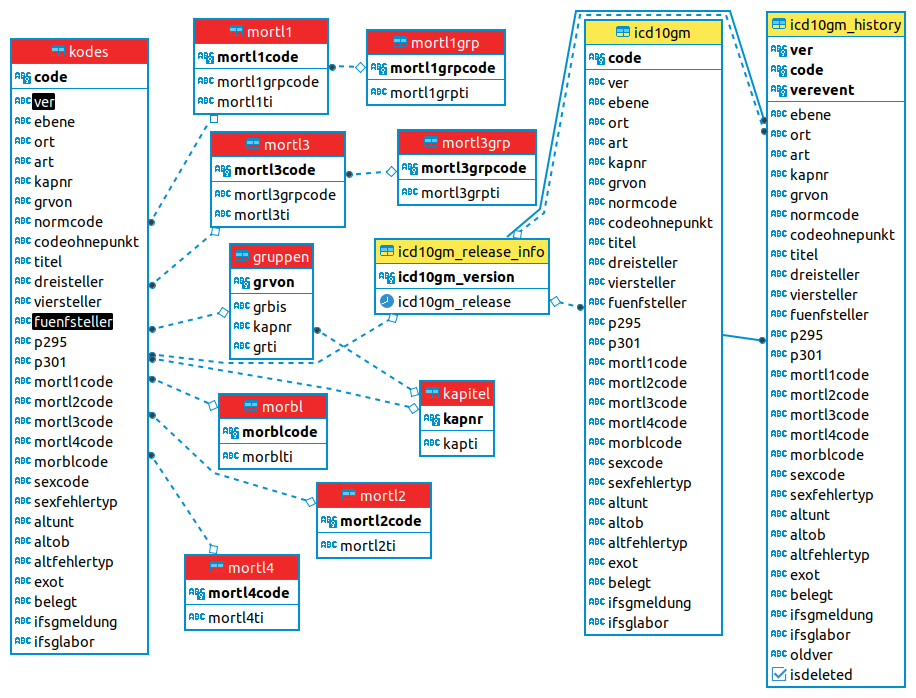
\includegraphics[height=10cm]{figures/icdSqlSchema}
	\caption[Datenbankstruktur]{Datenbankstruktur für die Steuerung der \ac{icd10gm}. Die Tabellen von \ac{bfarm} sind mit Kopfzeilen in rot gekennzeichnet, die Spalten in schwarz in diesen Tabellen sind die vorgenommenen Erweiterungen und Modifikationen. Die Tabellen mit Kopfzeilen in gelb sind die neuen eingeführten Tabellen für die Historisierung der \ac{icd10gm}.}
	\label{fig:reldb2}
\end{figure}

\subsection{Neue Tabellen} \label{subsec:newtables}

Für die Erfassung der Datierung der Veröffentlichungen der Versionen wurde die Tabelle \glqq\textsf{icd10gm\_release\_info}\grqq{} erstellt. Diese speichert den Identifikator oder das Jahr der Version in der Spalte \glqq\textsf{icd10gm\_version}\grqq{} als Hauptschlüssel und das Datum der Veröffentlichung in der Spalte \glqq\textsf{icd10gm\_release}\grqq{}. Diese hat das Format \glqq\textsf{JJJJ-MM-TT}\grqq{}. Wobei \glqq J\grqq{} das Jahr, \glqq M\grqq{} den Monat und \glqq T\grqq{} den Tag darstellen.

Die \ac{icd10gm} von 2007 bis 2021, werden in der Tabelle \glqq\textsf{icd10gm}\grqq{} gespeichert. In dieser Tabelle wird die Information der noch gültigen \ac{icd10gm} aktualisiert. Die gelöschten \ac{icd10gm} beinhalten die Information der letzten Aktualisierung. Die Spalte \glqq\textsf{code}\grqq{} dieser Tabelle ist der Hauptschlüssel, genau wie in der Tabelle \glqq\textsf{kodes}\grqq{} vom \ac{bfarm}-Schema. Das Feld \glqq\textsf{ver}\grqq{} speichert den Identifikator der Version der Insertion oder der letzten Änderung und ist ein Fremdschlüssel, der zu der Spalte \glqq\textsf{icd10gm\_version}\grqq{} der Tabelle \glqq\textsf{icd10gm\_release\_info}\grqq{} zeigt.

Die Tabelle \glqq\textsf{icd10gm\_history}\grqq{} enthält die Information der \ac{icd10gm}, die im Laufe der Zeit eingefügt, gelöscht oder geändert wurden. Die Besonderheiten diese Tabelle sind die Spalten \glqq\textsf{ver}\grqq{}, \glqq\textsf{oldver}\grqq{} und \glqq\textsf{verevent}\grqq{}. Die Identifikatoren vergangener Versionen einer \ac{icd10gm} werden in der Spalte \glqq\textsf{oldver}\grqq{} gespeichert. Die Spalte \glqq\textsf{ver}\grqq{} enthält den Identifikator der Fassungen bei deren eine \ac{icd10gm} eingefügt, gelöscht oder modifiziert wurde. Die Ereignisse einer Insertion, Änderung, Löschung oder Wiederverwendung werden mit den Buchstaben \glqq\textsf{I}\grqq{} (insert), \glqq\textsf{U}\grqq{} (update), \glqq\textsf{D}\grqq{} (delete) und \glqq\textsf{DI}\grqq{} (delete insert) in der Spalte \glqq\textsf{verevent}\grqq{} kodiert und gespeichert.

\section{Fluss der Information} \label{sec:dbrun}

Mit Hilfe einer \ac{etl}-Strecke werden die Daten aus der \ac{zip}-Datei in der \ac{db} importiert. Die Information der Veröffentlichung der \ac{icd10gm} wird in der Tabelle \glqq\textsf{icd10gm\_release \_info}\grqq{} eingefügt. Bei jedem Laden wird die Information der Tabelle \glqq\textsf{kodes}\grqq{} vorher gelöscht und mit neuen Datensätzen geladen. 

Die Kodes, die vorher nicht in der Tabelle \glqq\textsf{icd10gm}\grqq{} vorhanden waren, werden in diese und in die Tabelle \glqq\textsf{icd10gm\_history}\grqq{} kopiert. Diese Datensätze werden in \glqq\textsf{icd10gm\_history}\grqq{} als eingefügt markiert. 

Nicht in \glqq\textsf{kodes}\grqq{} existierende \ac{icd10gm} werden aus \glqq\textsf{icd10gm}\grqq{} in \glqq\textsf{icd10gm\_history}\grqq{} kopiert. Diese Kopie wird als gelöscht markiert, und enthält die Indikatoren der Fassung der Insertion oder der letzten Änderung in der Spalte \glqq\textsf{oldver}\grqq{}, und der Fassung der Löschung in der Spalte \glqq\textsf{ver}\grqq{}. 

Existierende Kodierungen mit modifizierten Informationen werden in der Tabelle \glqq\textsf{icd10gm}\grqq{} aktualisiert und nachher in \glqq\textsf{icd10gm\_history}\grqq{} hinzugefügt. In diesem Fall werden auch die Indikatoren der alten und neuen Fassung registriert und der Datensatz als modifiziert markiert.

Dieser Fluss der Information ist im Datenflussdiagramm der Abbildung~\ref{fig:dbflow} repräsentiert. Der automatisierte Prozessablauf in der \ac{db} ist durch Trigger in den Tabellen \glqq\textsf{kodes}\grqq{} und \glqq\textsf{icd10gm}\grqq{} gesteuert.

\begin{figure}[ht]
	\centering
	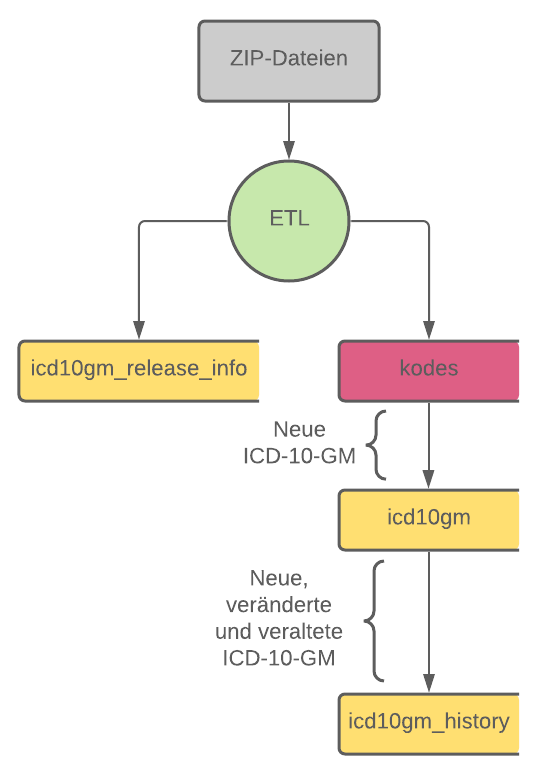
\includegraphics[height=10cm]{figures/dbflow}
	\caption[Datenfluss des Prozesses]{Datenflussdiagramm der Informationen von den \ac{zip}-Dateien bis zum Import in der \ac{db}.}
	\label{fig:dbflow}
\end{figure} 
	%\newpage
	\section{\acs{etl}-Strecke} \label{sec:etlpipeline}

Für den Import der Information der \ac{icd10gm} in der \ac{db} wurde eine \ac{etl}-Strecke entwickelt. Dazu wurden \ac{bash}-Skripts unter Ubuntu 20.04 programmiert und durchgeführt. Die Entscheidung von \ac{bash} basiert sich darauf, dass \ac{bash} die Standard interaktive Shell und Skript Sprache von Linux-Betriebssystemen ist und ermöglicht auch die Automatisierung einer Reihenfolge von Kommandos des Betriebssystems \cite{bash}. Da die Interaktion mit den Befehlen des Betriebssystems via \ac{bash} effizienter und leichter ist, ist es möglich in einer sicheren Art die Zugangsdaten für die \ac{db} zu nutzen, ohne diese Information in Klartext in den Skripten oder in anderen Dateien sichtbar zu platzieren.

Der Anfangspunkt für die Durchführung der \ac{etl} sind die \ac{zip}-Dateien der \ac{icd10gm} Metadaten von 2007 bis 2021 aus der Download Seite vom \ac{bfarm} für die Klassifikationen. Diese Dateien wurden zuerst manuell heruntergeladen. Der Abruf und die Reihenfolge der Skripts für den Durchlauf jedes Schritts der \ac{etl} werden von einem zentralen \ac{bash}-Skript definiert. Die Abbildung~\ref{fig:etl} stellt das Flussdiagramm der \ac{etl}-Strecke dar.

\clearpage
\begin{figure}[ht]
	\centering
	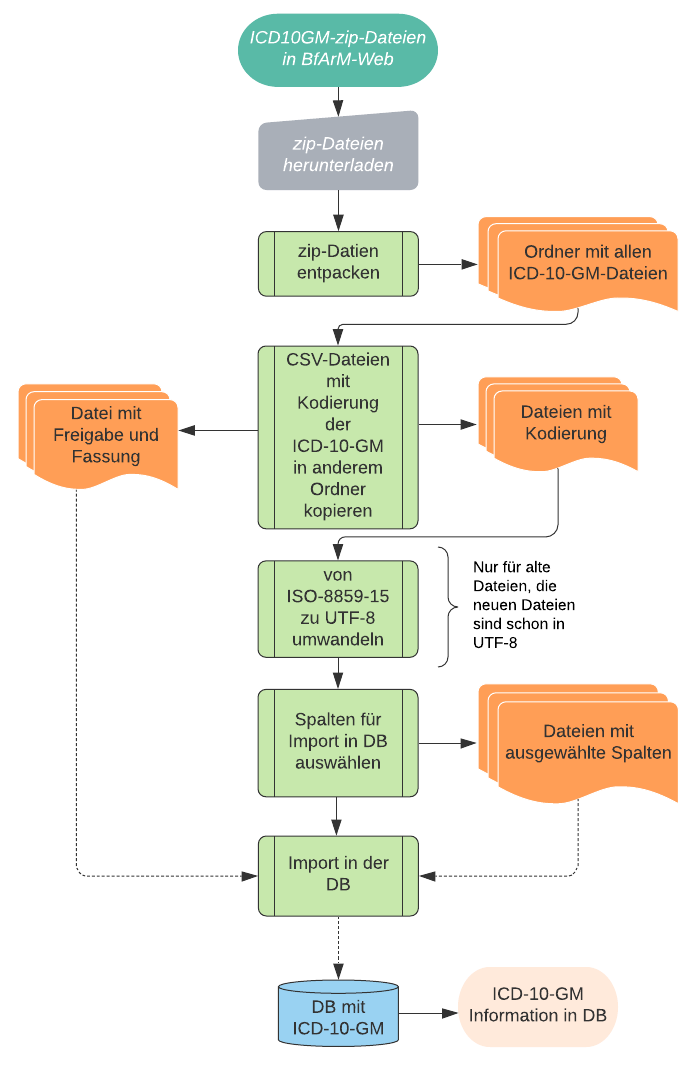
\includegraphics[height=14cm]{figures/etl}
	\caption[\acs{etl}-Strecke]{Flussdiagramm der \acs{etl}-Strecke für den Import der Informationen der \ac{icd10gm} aus den \ac{zip}-Dateien in der \ac{db}.}
	\label{fig:etl}
\end{figure} 

\subsection{Extraktion} \label{subsec:extraction}

Zuerst werden die Ordner der \ac{zip}-Dateien entpackt und ein neuer Ordner für die Speicherung der Kode-Dateien wird generiert. Diese Dateien werden ausgewählt und in den hergestellten Ordner kopiert. Die Information des Datums der Freigabe und Fassung wird aus der Liesmich-Datei extrahiert und in einer \ac{csv}-Datei importiert.

%Zuerst werden die Ordner der \ac{zip}-Dateien mit Hilfe des Skripts \textsf{unzipper.sh} entpackt. Das Skript \textsf{copy\_codes.sh} generiert ein neuen Ordner für die Speicherung der Kode-Dateien. Diese Dateien werden ausgewählt und in diesem Ordner kopiert. Die Information des Datums der Freigabe und Fassung wird mit dem Skript \textsf{extra\_info.sh} aus der Liesmisch-Dateien extrahiert und in einem \ac{csv}-Datei importiert.

\subsection{Transformation} \label{subsec:transf}

Die Kode-Dateien von 2007 bis 2009 haben den Windows-Standardzeichensatz \acl{iso}, \acsu{iso}-8859-15 als Zeichenkodierung. Das verursacht Probleme bei dem Datenaustausch zwischen Plattformen, da die PostgreSQL Instanz in \acl{utf}, \acsu{utf}-8 konfiguriert ist. Aus diesem Grund wird das Format dieser Kode-Dateien von \ac{iso}-8859-15 in \ac{utf}-8 umgewandelt.

Im Laufe der Zeit sind neue Spalten in der \ac{csv}-Dateien der Klassifizierungen entstanden und andere Felder werden veraltet und entnommen \cite{readme13, readme17}. Deswegen werden die aktuell benutzten Spalten ausgewählt, leere Felder werden an den Positionen der Spalten die vorher nicht vorhanden waren eingefügt, ein neues Feld mit der Version am Anfang jede Zeile ist eingeführt, und der Datensatz mit den Änderungen in einer neuen generierten \ac{csv}-Datei gespeichert.
%Die Kode-Dateien von 2007 bis 2009 haben den Windows-Standardzeichensatz (ISO-8859-15) als Zeichenkodierung. Das verursacht Probleme bei dem Datenaustausch zwischen Plattformen. Aus diesem Grund wandelt das Skript \textsf{iso\_2\_utf8.sh} das Format dieser Kode-Dateien von ISO-8859-15 in UTF-8 um.

%Mit der Laufe der Zeit sind neue Spalten in der \ac{csv}-Dateien entstanden und andere Felder werden veraltet und entnommen \cite{readme13, readme17}. Deswegen das Skript \textsf{select\_columns.sh}, wählt die aktuell benutzte Spalten aus, fügt leere Felder an der Positionen die vorher nicht vorhanden waren ein, fügt ein neues Feld mit der Version an Anfang jede Zeile ein, und importiert der Datensatz einer neuen generierten \ac{csv}-Dateien.

\subsection{Laden} \label{subsec:load}

Am Ende der Transformation wird die Information der zuletzt generierten \ac{csv}-Dateien mit Kodes in der Tabelle \glqq\textsf{kodes}\grqq{} der \ac{db}. Der interne Datenfluss in der \ac{db} ist in der Sektion~\ref{sec:dbrun} beschrieben.
	%\newpage
	\chapter{Ergebnisse} \label{ch:results}

\section{\acs{icd10gm} in der \acs{csv}-Dateien und \acs{db}} \label{sec:dataanalysis}
Die Analyse der Information der \ac{icd10gm} wurde mit Hilfe von \ac{sql}-Befehlen und der Skript Sprache Python unter dem Framework Jupyter-Notebook durchgeführt.

Wie in der Tabelle~\ref{tab:icdfiles} dargestellt wird, jede Kode-Datei enthält mehr als 15450 Kodes, obwohl manche Kodierungen gelöscht werden, nimmt die Menge neuer \ac{icd10gm} ständig zu.

\begin{table}[ht]
	\centering
	\small
	\caption[\acs{icd10gm} in den \acs{csv}-Dateien]{Anzahl an \acs{icd10gm} pro Jahr in den \ac{csv}-Dateien}
	\label{tab:icdfiles}
	\begin{tabular}{|l|l|}
		\hline
	\rowcolor{lightgray} Anzahl & Fassung \\ \hline 
		15455 & 2007 \\ \hline
		15498 & 2008 \\ \hline
		15523 & 2009 \\ \hline
		15598 & 2010 \\ \hline
		15633 & 2011 \\ \hline
		15643 & 2012 \\ \hline
		15668 & 2013 \\ \hline
		15688 & 2014 \\ \hline
		15761 & 2015 \\ \hline
		15821 & 2016 \\ \hline
		15930 & 2017 \\ \hline
		16059 & 2018 \\ \hline
		16126 & 2019 \\ \hline
		16131 & 2020 \\ \hline
		16203 & 2021 \\ \hline
		\hline
		236737 & \textbf{Gesamt} \\ \hline
	\end{tabular}
	\end{table}

Nach dem Durchlauf der \ac{etl} sind insgesamt 16520 \ac{icd10gm} von 2007 bis 2021 in der \ac{db} eingefügt. In der Abbildung~\ref{fig:icddb} ist das Verhältnis dieser Kodierungen in Bezug auf die Modifikationen dargestellt. Die konkreten Zahlen dieser Modifikationen sind in der Tabelle~\ref{tab:icdupd} dargestellt. 
 
 \begin{figure}[ht]
 	\centering
 	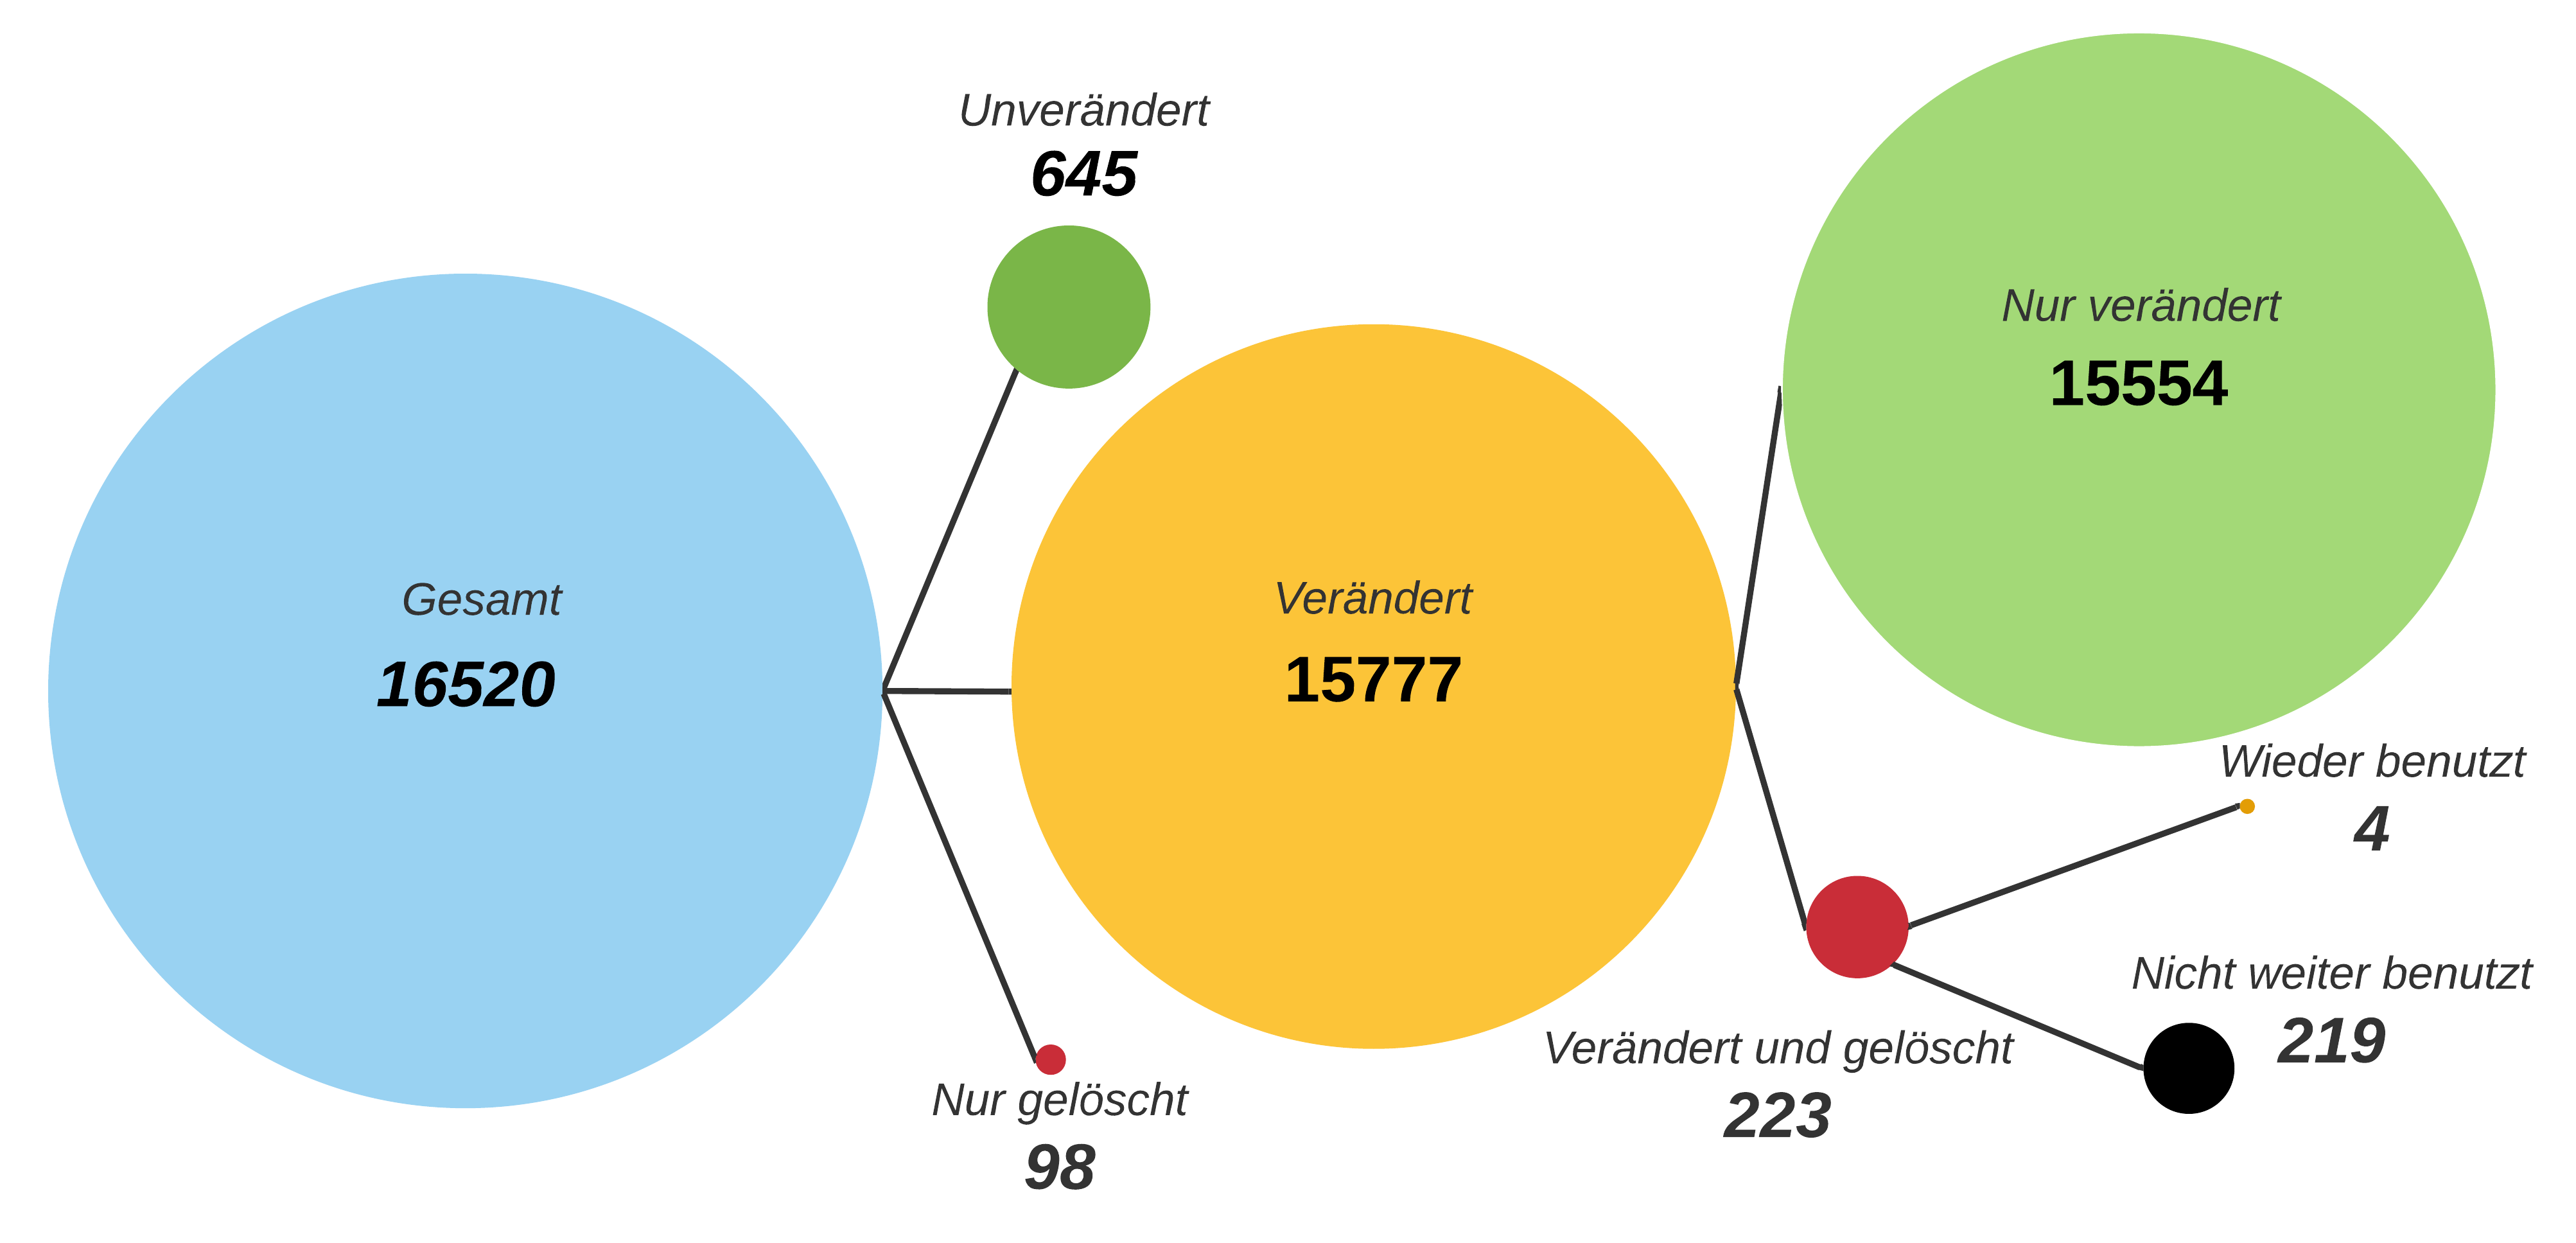
\includegraphics[height=6cm]{figures/icd10gm_quantities}
 	\caption[\acs{icd10gm} in der \acs{db}]{Charakterisierung der \acs{icd10gm} in der \ac{db} in Bezug auf die Modifikationen.}
 	\label{fig:icddb}
 \end{figure}

\section{Zeitliche Entwicklung der \acs{icd10gm}} \label{sec:timeicd}

Die Darstellung der Besonderheiten eines Lebenszyklus der historischen \ac{icd10gm} Auffassungen ist in der Tabelle~\ref{tab:IUDDI} exemplarisch dargestellt. Das Beispiel zeigt die chronologische Entwicklung der \ac{icd10gm} in der Tabelle \glqq\textsf{icd10gm\_history}\grqq{} der \ac{db}. Die Spalte Fassung, \glqq\textsf{ver}\grqq{} in der Tabelle \glqq\textsf{icd10gm\_history}\grqq{}, zeigt die Version der Einführung, Änderung, Löschung oder Wiederverwendung einer \ac{icd10gm}. Das Feld Alte Fassung, \glqq\textsf{oldver}\grqq{} in der vorher genannten Tabelle, beinhaltet den Identifikator der vorherigen Fassung einer Schlüsselnummer. In der Spalte Ereignis, \glqq\textsf{verevent}\grqq{} in der Tabelle \glqq\textsf{icd10gm\_history}\grqq{}, sind die Ereignisse Einführung, Änderung, Löschung und Wiederverwendung, wie in der Subsektion~\ref{subsec:newtables} beschrieben wurden, kodiert. Eine wichtige Anmerkung in der Darstellung ist, dass die gezeigte alte Fassung bei der wiederverwendeten Klassifikationen, die Version der Insertion oder der letzten Änderung ist, weil dieser Kode in der Fassung der Löschung nicht vorhanden war.

Somit könnten wir erkennen, dass unsere Implementierung die Lebenszyklus von \ac{icd10gm} Klassifikationen darstellen kann, sodass jede Modifikation in der Semantik zwischen 2007 und 2021 dokumentiert ist. In den weiteren Sektionen werden die verschiedenen Änderungen in dem semantischen Verzeichnis und einigen Sonderverzeichnissen gezeigt und deren Gründe erklärt.
%\clearpage

\begin{table}[ht]
	\centering
	\small
	\caption[Beispiel der Historisierung einer \acs{icd10gm} Klassifikation]{Beispiel der Historisierung einer \acs{icd10gm} Klassifikation. Diese stellt eine, nach der Einführung, veränderte, gelöschte, und wieder benutzte Schlüsselnummer dar.}
	\label{tab:IUDDI}
	\begin{tabular}{|l|l|p{6cm}|l|l|}
		\hline
		\rowcolor{lightgray} Fassung & Kode & Titel & Alte Fassung & Ereignis \\ \hline
		2007 & N90.8  & Sonstige näher bezeichnete nichtentzündliche Krankheiten der Vulva und des Perineums &  & I \\ \hline
		2008 & N90.8  & Sonstige näher bezeichnete nichtentzündliche Krankheiten der Vulva und des Perineums & 2007 & U \\ \hline
		2013 & N90.8  & Sonstige näher bezeichnete nichtentzündliche Krankheiten der Vulva und des Perineums & 2008 & U \\ \hline
		2014 & N90.8  & Sonstige näher bezeichnete nichtentzündliche Krankheiten der Vulva und des Perineums & 2013 & D \\ \hline
		2016 & N90.8  & Sonstige näher bezeichnete nichtentzündliche Krankheiten der Vulva und des Perineums & 2013 & DI \\ \hline
	\end{tabular}
\end{table}

\section{Neue \acs{icd10gm}} \label{sec:newicd}

Von 2008 bis 2021 sind insgesamt 966 neue \ac{icd10gm} entstanden. In der Abbildung~\ref{fig:newicdyear} ist ein interessanter Aspekt davon repräsentiert, nämlich die Anzahl neuer \ac{icd10gm} pro Jahr ist unregelmäßig. Es gib Jahre wie 2017 und 2018 mit mehr als 120 neuen Einträgen. Dieses Phänomen passiert am meisten beim Bedarf neuer Subklassifikationen, um die Diagnosen spezifischer zu kodieren und an diverse klinische Systeme anzupassen. Ein Beispiel dieses Phänomens ist der Kode \textsf{U81!} \textsf{Bakterien mit Multiresistenz gegen Antibiotika}, dieser wurde 2017 entnommen und stattdessen entstand die Kodierung \textsf{U81.-!} \textsf{Gramnegative Erreger mit bestimmten Antibiotikaresistenzen, die besondere therapeutische oder hygienische Maßnahmen erfordern} zusammen mit 43 weiteren Subklassifikationen von \textsf{U81.0-!} bis \textsf{U81.8!}. Die Ursache davon war eine Umstrukturierung der Bereiche \textsf{U81!}, um diese Kodes an die Nomenklatur der \ac{krinko} anzupassen~\cite{erreg17}.

Im Jahr 2018 wurden mehr als 80 neue \ac{icd10gm} in den Bereichen \textsf{M14.-*} \textsf{Arthropathien bei sonstigen anderenorts klassifizierten Krankheiten} eingefügt. Diese Zunahme ist auch in der Abbildung~\ref{fig:newicdcap} widerspiegelt, denn diese Diagnosen sind im Kapitel \textsf{Krankheiten des Muskel-Skelett-Systems und des Bindegewebes} repräsentiert. Die Ursache dieser Zunahme war die Insertion einer fünften Stelle an der Kodierung, um die Abbildung im \ac{gdrg}-System zu ermöglichen~\cite{musk18}.

%\clearpage

\begin{figure}[ht]
	\centering
	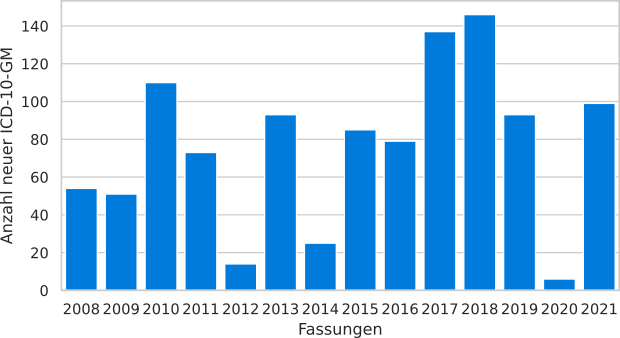
\includegraphics[height=7cm]{figures/newicdyear}
	\caption[Neue \acs{icd10gm} pro Jahr]{Anzahl neuer \acs{icd10gm} zwischen den Jahren 2008 und 2021}
	\label{fig:newicdyear}
\end{figure} 

Ein wichtiger und aktueller Punkt sind die meldepflichtigen Krankheiten im Laufe der Jahre. Dieses Phänomen ist in der Abbildung~\ref{fig:newicdmeld} dargestellt. Es ist zu erkennen, dass neue meldepflichtige Kodes in den Jahren 2010, 2016 und 2021 definiert wurden (Tabelle~\ref{tab:meldung}). Ursachen davon sind Pandemien und Epidemien wie die Influenza Varianten zwischen 2009 und 2010~\cite{influenza1, influenza2}, die Verbreitung des Dengue Fiebers in Europa als Effekt der Globalisierung mit der steigenden Mobilität~\cite{denge1} und Verbreitung der asiatischen Tigermücke \textsl{Aedes (Stegomyia) albopictus} zwischen 2015 und 2016 in der Region als Konsequenz der milden Winter~\cite{denge2}, und noch aktuell seit Februar 2020 die Verbreitung des Corona Virus in Europa~\cite{corona1} und deren gesundheitlichen Folgen~\cite{corona2}. 

Ein interessanter Aspekt der meldepflichtigen Krankheiten in der Tabelle~\ref{tab:meldung} ist die Diagnose \textsf{B17.9} \textsf{Akute Virushepatitis, nicht näher bezeichnet}. Diese Krankheit war unter \textsf{K72.0} \textsf{Akutes und subakutes Leberversagen} zugeordnet, erst 2010 wurde zur Kenntnis genommen, dass es sich bei der akuten Hepatitis in manchen Fällen um eine akute infektiöse Hepatitis handelt. Aus diesem Grund hatte die \ac{who} die Schlüsselnummer \textsf{B17.9} zur Verfügung gestellt~\cite{komm10}.

\clearpage

\begin{figure}[ht]
	\centering
	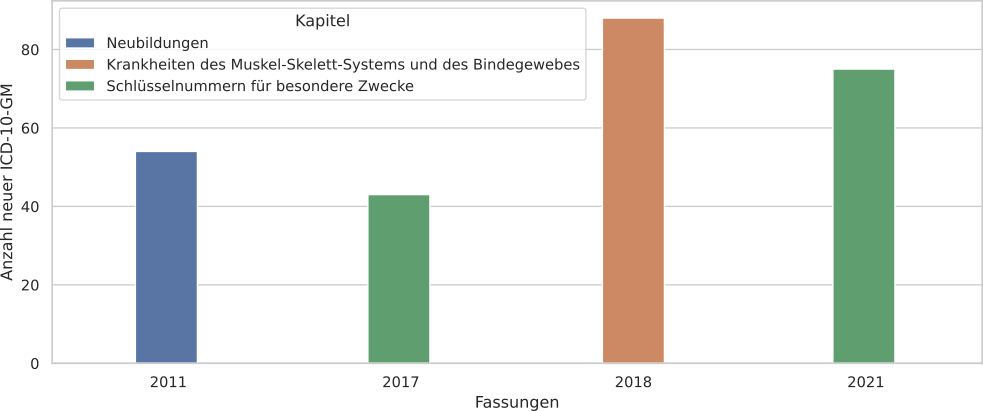
\includegraphics[height=5.7cm]{figures/kaptnrYear}
	\caption[Kapitel mit den meisten eingeführten \acs{icd10gm} (2008 - 2021)]{Kapitel mit den meisten neuen Kodierungen zwischen 2008 und 2021}
	\label{fig:newicdcap}
\end{figure}

%\clearpage
\begin{figure}[ht]
	\centering
	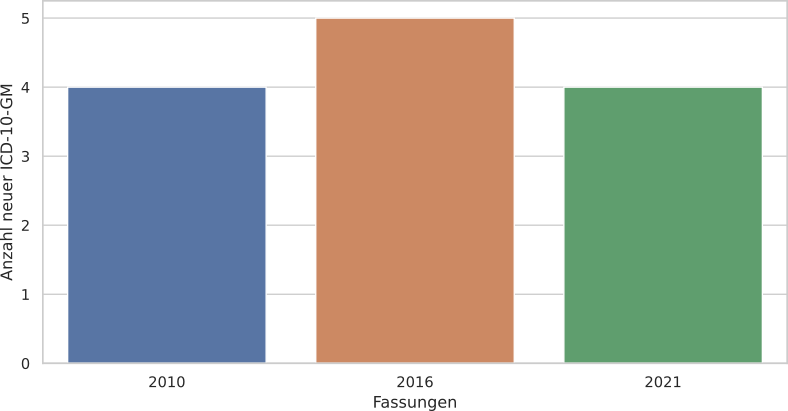
\includegraphics[height=5.7cm]{figures/arztJaYear}
	\caption[Neue meldepflichtige \acs{icd10gm} pro Jahr]{Menge der neuen meldepflichtigen Diagnosen zwischen den Jahren 2008 und 2021}
	\label{fig:newicdmeld}
\end{figure} 

\clearpage
\begin{table}[ht]
	\centering
	\small
	\caption[Meldepflichtige \acs{icd10gm}]{Meldepflichtige Krankheiten}
	\label{tab:meldung}
	\begin{tabular}{|l|l|p{10.5cm}|}
		\hline
		\rowcolor{lightgray} Fassung & \acs{icd10gm} & Titel \\ \hline
		2010 & B17.9 & Akute Virushepatitis, nicht näher bezeichnet \\ \hline
		2010 & U69.2-! & Sekundäre Schlüsselnummern für besondere epidemiologische Zwecke \\ \hline
		2010 & U69.20! & Influenza A/H1N1 Pandemie 2009 [Schweinegrippe] \\ \hline
		2010 & U69.21! & Influenza A/H5N1 Epidemie [Vogelgrippe] \\ \hline
		2016 & A97.- & Dengue \\ \hline
		2016 & A97.0 & Dengue ohne Warnzeichen \\ \hline
		2016 & A97.1 & Dengue mit Warnzeichen \\ \hline
		2016 & A97.2 & Schweres Dengue \\ \hline
		2016 & A97.9 & Dengue, nicht näher bezeichnet \\ \hline
		2021 & U07.1! & COVID-19, Virus nachgewiesen \\ \hline
		2021 & U07.2! & COVID-19, Virus nicht nachgewiesen \\ \hline
		2021 & U10.- & Multisystemisches Entzündungssyndrom in Verbindung mit COVID-19 \\ \hline
		2021 & U10.9 & Multisystemisches Entzündungssyndrom in Verbindung mit COVID-19, nicht näher bezeichnet \\ \hline
	\end{tabular}
\end{table}

\section{Modifizierte \acs{icd10gm}} \label{sec:updicd}

Jedes Jahr werden Änderungen in den Metadaten der \ac{icd10gm} vorgenommen. Solche Modifikationen sind in der Tabelle \ref{tab:icdupd} aufgelistet. Wie in der Sektion~\ref{sec:dataanalysis} genannt wurde, sind die meisten Änderungen an den Spalten für die dritten, vierten und fünften Stellen  der Kodes, weil diese Felder erst im Jahr 2013 entstanden sind~\cite{readme13}. Ein weiterer Aspekt in Bezug auf die zahlreichen Änderungen ist, dass die Werte verschiedener Felder bei manchen \ac{icd10gm} in früheren Fassungen noch nicht definiert waren, wie in der Tabelle~\ref{tab:icdupd} in den Fällen der Mortaliätslisten verdeutlicht wird. Die Werte solcher Listen bei den meisten Kodes im Jahr 2007 waren nicht definiert, und waren mit dem Wert \glqq\textsf{UNDEF}\grqq{} gesetzt. Erst 2008 wurden diese Felder durch einen spezifischen Wert ersetzt. Die zahlreichen Modifikationen an den Klassentiteln sind durch Vorschläge zur Weiterentwicklung der Klassifikationen entstanden~\cite{diab09, komm14}. 
%  Ein Beispiel davon ist die Schlüsselnummer \textsf{E10.31} mit dem Titel \textsf{Primär insulinabhängiger Diabetes mellitus [Typ-1-Diabetes] \underline{mit} Augenkomplikationen: Als entgleist bezeichnet}. Dieser Titel wurde zu \textsf{Primär insulinabhängiger Diabetes mellitus [Typ-1-Diabetes] \underline{: Mit } Augenkomplikationen: Als entgleist bezeichnet} in 2009 geändert. Die Änderung wurde in diesem Jahr durchgeführt, da eine fünfte Stelle in der Klassifikationen von \textsf{E10}  bis \textsf{E14} eingefügt wurde~\cite{diab09}. Der Titel dieser \ac{icd10gm} wurde nochmal in 2014 zu \textsf{\underline{Diabetes mellitus, Typ 1: Mit Augenkomplikationen: Als entgleist bezeichnet}} ersetzt. In diesem Jahr wurden die Titel von der \ac{who} an die gebräuchliche Terminologie angepasst~\cite{komm14}.

%\clearpage

\begin{table}[ht]
	\centering
	\small
	\caption[Änderungen in den Metadaten]{Liste der Metadaten und Anzahl an Änderungen}
	\label{tab:icdupd}
	\begin{tabular}{|l|p{11.5cm}|}
		\hline
		\rowcolor{lightgray} Änderungen & Metadaten \\ \hline
		15578 & Dritte Stelle \\ \hline
		13871 & Vierte Stelle \\ \hline
		6949 & Bezug zur Mortalitätsliste 3 \\ \hline		
		6348 & Bezug zur Mortalitätsliste 1 \\ \hline
		2 & \textbf{Bezug zur Mortalitätsliste 1 (definiert)} \\ \hline
		5061 & Fünfte Stelle \\ \hline
		%1193 & Art des Fehlers bei Geschlechtsbezug \\ \hline
		1111 & Klassentitel \\ \hline
		308 & Untere Altersgrenze \\ \hline
		36 & \textbf{Untere Altersgrenze (relevant)} \\ \hline
		299 & Bezug zur Morbiditätsliste \\ \hline
		11 & \textbf{Bezug zur Morbiditätsliste (definiert)} \\ \hline
		%286 & Alter Fehlertyp \\ \hline
		286 & Obere Altersgrenze \\ \hline
		14 & \textbf{Obere Altersgrenze (relevant)} \\ \hline
		162 & Anwendung der Laborausschlussziffer des \ac{ebmg} \\ \hline
		118 & Art der Vier- und Fünfsteller \\ \hline
		69 & Bezug zur Mortalitätsliste 4 \\ \hline
		68 & Geschlechtsbezug \\ \hline
		64 & Bezug zur Mortalitätsliste 2 \\ \hline
		2 & \textbf{Bezug zur Mortalitätsliste 2 (definiert)} \\ \hline
		44 & Kategorie der Gruppe \\ \hline
		40 & Arzt-Meldepflicht \\ \hline		
		31 & Sehr seltene Krankheit in Mitteleuropa \\ \hline				
		6 & Belegung des Kodes \\ \hline
		3 & \S 295 \ac{sgb} V \\ \hline		
		2 & Klassifikationsebene \\ \hline
		
	\end{tabular}
\end{table}

Ein interessanter Aspekt an der Stelle des Geschlechtsbezugs ist, dass 52 Diagnosen mit Geschlechtsbezug der 68 an dieser Stelle geänderten Schlüsselnummer, Krankheiten der Brustdrüse sind. Diese \ac{icd10gm} waren früher auf das weibliche Geschlecht bezogen, jetzt ist der Geschlechtsbezug dieser Kodierungen irrelevant. Viele dieser Änderungen wurden in den Jahren 2008 und 2016 vorgenommen. An dieser Stelle können wir nicht erklären, wieso diese Art von Krankheiten nicht immer ohne Geschlechtsbezug waren, denn seit 1930 existieren medizinische Publikationen über Brustdrüsen Anomalien bei Männern~\cite{bcm}. In den heutigen Tagen gibt es eine leichte Zunahme an Männern mit Brustkrebs~\cite{giobcm} und die erste deutschsprachige Fassung der ICD-10 für die Zwecke des \ac{sgb} V wurde schon 1996 erarbeitet~\cite{icdgmhistory}.

\clearpage

\begin{table}[ht]
	\centering
	\caption[Beispiel von seltenen Krankheiten in Mitteleuropa (Diphtherie und Poliomyelitis)]{Beispiel von seltenen Krankheiten in Mitteleuropa anhand von \ac{icd10gm} der Bereiche \textsf{A36.-} \textsf{Diphtherie} und \textsf{A80.-} \textsf{Akute Poliomyelitis [Spinale Kinderlähmung]}. Die alten und neuen Werte sind in der Spalte \glqq Alt\grqq{} bzw. \glqq Neu\grqq{}. \glqq\textsf{N}\grqq{} Nein, \glqq\textsf{J}\grqq{}\grqq{} Ja.}
	\label{tab:icdeuropa}
	\begin{tabular}{|p{1.6cm}|l|p{7cm}|l|l|}
		\hline
		\rowcolor{lightgray} Fassung der Änderung & \ac{icd10gm} & Titel & Alt & Neue \\ \hline
		\rowcolor{maroon!10} 2011 & A36.- & Diphtherie & N & J \\ \hline
		2011 & A36.0 & Rachendiphtherie & N & J \\ \hline
		2011 & A36.1 & Nasenrachendiphtherie & N & J \\ \hline
		2011 & A36.2 & Kehlkopfdiphtherie & N & J \\ \hline
		2011 & A36.3 & Hautdiphtherie & N & J \\ \hline
		2011 & A36.8 & Sonstige Diphtherie & N & J \\ \hline
		2011 & A36.9 & Diphtherie, nicht näher bezeichnet & N & J \\ \hline \hline
		\rowcolor{maroon!10} 2011 & A80.- & Akute Poliomyelitis [Spinale Kinderlähmung] & N & J \\ \hline
		2011 & A80.0 & Akute paralytische Poliomyelitis durch Impfvirus & N & J \\ \hline
		2011 & A80.1 & Akute paralytische Poliomyelitis durch importiertes Wildvirus & N & J \\ \hline
		2011 & A80.2 & Akute paralytische Poliomyelitis durch einheimisches Wildvirus & N & J \\ \hline
		2011 & A80.3 & Sonstige und nicht näher bezeichnete akute paralytische Poliomyelitis & N & J \\ \hline
		2011 & A80.4 & Akute nichtparalytische Poliomyelitis & N & J \\ \hline
		2011 & A80.9 & Akute Poliomyelitis, nicht näher bezeichnet & N & J \\ \hline
	\end{tabular}
\end{table}

Von den sehr seltenen Krankheiten in Mitteleuropa sind 20 der 31 Diagnosen belegte Schlüsselnummern, also Kodierungen ohne Unterkategorien und somit im alltäglichen  Gebrauch. Davon gehören 12 zu den Bereichen \textsf{A36.-} \textsf{Diphtherie} und \textsf{A80.-} \textsf{Akute Poliomyelitis [Spinale Kinderlähmung]}. Diese sind in der Tabelle~\ref{tab:icdeuropa} aufgelistet. Diese Diagnosen sind heutzutage selten, Ursache ist die erfolgreiche Impfkampagne in Deutschland, sodass die vom \ac{rki} jährlich selten gemeldeten Fällen in den heutigen Tagen importiert sind~\cite{dippol1}.

\section{Gelöschte \acs{icd10gm}} \label{sec:deletedicd}

In jeder Fassung von 2008 bis 2021 werden \ac{icd10gm} gelöscht. Dieses Verhalten ist in der Abbildung~\ref{fig:newdeleteoldicdyear} repräsentiert. Die meisten Schlüsselnummern wurden im Jahr 2013 gelöscht, da eine umfangreiche Umstrukturierung in der Semantik in diesem Jahr vorgenommen wurde. Die Kapitel, die in diesem Jahr am meisten betroffen waren, sind in der Abbildung~\ref{fig:kap13} dargestellt. Bei der semantischen Umstrukturierung im Jahr 2013 wurden bestimmte Kodebereiche im Kapitel \textsf{Krankheiten des Kreislaufsystems} umfänglich überarbeitet, viele fünfstellige Klassifizierungen wurden vom Kapitel \textsf{Krankheiten des Muskel-Skelett-Systems und des Bindegewebes} entnommen, und im Kapitel \textsf{Schlüsselnummern für besondere Zwecke} wurden zahlreiche \ac{icd10gm} umgebaut~\cite{dele13}.

%\clearpage
\begin{figure}[ht]
	\centering
	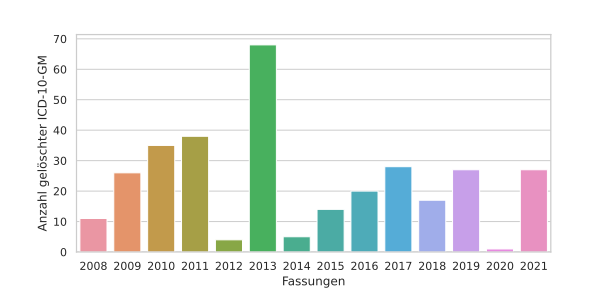
\includegraphics[height=6cm]{figures/neuVersionDelete}
	\caption[Gelöschte \acs{icd10gm} pro Jahr]{Anzahl gelöschter \acs{icd10gm} zwischen den Jahren 2008 und 2021}
	\label{fig:newdeleteoldicdyear}
\end{figure} 

\clearpage

\begin{figure}[ht]
	\centering
	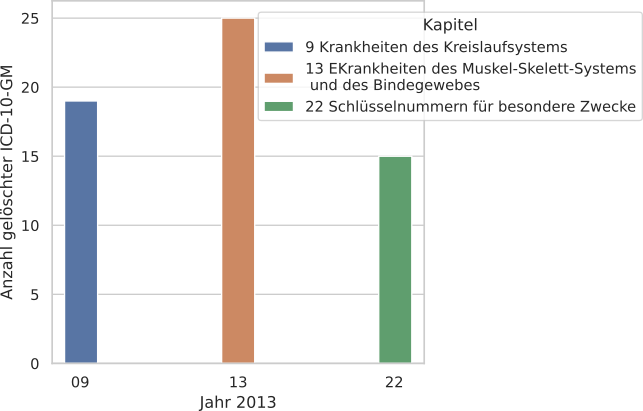
\includegraphics[height=6cm]{figures/kaptnr13}
	\caption{Meist betroffene Kapitel beim Löschen 2013}
	\label{fig:kap13}
\end{figure}


Die Abbildung \ref{fig:oldicdort} zeigt, dass die meisten Kodes, nämlich 295 der 321 gelöschten Kodierungen, terminale Schlüsselnummer waren, also \ac{icd10gm}, die in den Texten der Dokumentation der Diagnosen benutzt werden sollen. Von diesen terminalen Kodierungen wurden 115 erweitert, wie in der Sektion \ref{sec:newicd} Anhang des Beispiels von \textsf{U81!} erläutert wurde. Von den nicht terminalen Kodierungen wurden dann 11 erweitert. Ein Beispiel davon ist \textsf{Z75.2-} \textsf{Wartezeit auf eine Untersuchung oder Behandlung}. Diese nicht terminale Kodierung wurde gelöscht, und von dem terminalen Kode \textsf{Z75.2} mit demselben Titel ersetzt. 

%\clearpage

\begin{figure}[ht]
	\centering
	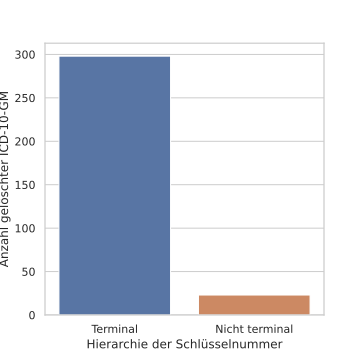
\includegraphics[height=6cm]{figures/ortoldYear}
	\caption{Hierarchie der gelöschten \acs{icd10gm}}
	\label{fig:oldicdort}
\end{figure}

%\newpage

\section{Wiederverwendete \acs{icd10gm}} \label{sec:delinicd}

Die Tabelle~\ref{tab:wieder} zeigt die 4 Schlüsselnummern, die wiederverwendet wurden.

\begin{table}[ht]
	\centering
	\small
	\caption[Wieder benutzte \acs{icd10gm}]{Liste der wieder benutzten Schlüsselnummern.}
	\label{tab:wieder}
	\begin{tabular}{|l|l|l|p{6cm}|}
		\hline
		\rowcolor{lightgray} Gelöscht & Wieder & \ac{icd10gm} & Aktueller Titel \\ \hline
		2013 & 2015 & M21.60 & Erworbener Hohlfuß [Pes cavus] \\ \hline
		2013 & 2015 & M21.6- & Sonstige erworbene Deformitäten des Knöchels und des Fußes \\ \hline
		2014 & 2016 & N90.8 & Sonstige näher bezeichnete nichtentzündliche Krankheiten der Vulva und des Perineums \\ \hline
		2010 & 2019 & K55.8 & Sonstige Gefäßkrankheiten des Darmes \\ \hline

\end{tabular}
\end{table}

Die Schlüsselnummern \textsf{M21.6-} und \textsf{M21.60} wurden 2013 entnommen, da im Kodebereich \textsf{M20-M25} zahlreiche Schlüssel zu keinen sinnvollen Kombinationen führten~\cite{dele13}. Andererseits wurde 2015 die Kategorie \textsf{M21.6} mit den genannten Schlüsselnummern wieder aufgenommen, um eine bessere Spezifikation der Diagnosen in dem \ac{gdrg}-System zu erreichen~\cite{komm15}. 

Die \ac{icd10gm} \textsf{N90.8} wurde 2014 entnommen und stattdessen wurde \textsf{N90.8-} \textsf{Sonstige näher bezeichnete nichtentzündliche Krankheiten der Vulva und des Perineums} mit weiteren Subklassifikationen zur spezifischen Kodierung eingeführt~\cite{komm14}. Zwei Jahre später, 2016, wurde der Kode \textsf{N90.8-} und deren Unterkategorien wieder entnommen und zu einem anderen Kapitel mit neuen Kodierungen verlagert, und die Schlüsselnummer \textsf{N90.8} wurde wieder eingeführt~\cite{komm16}.

Die Kodierungsschlüssel \textsf{K55.8} wurde 2010 gelöscht und die Kodierung \textsf{K55.8-} \textsf{Sonstige Gefäßkrankheiten des Darmes} mit weiteren Stellen eingeführt, um einige Diagnosen des Dünndarms besser abgrenzen zu können~\cite{komm10}. 2019 wurde die \ac{icd10gm} \textsf{K55.3-} \textsf{Angiodysplasie des Dünndarmes} mit weiteren fünfstelligen Kodes eingeführt und die, 2010, eingeführten Klassifikationen wurden auf den neuen Kodebereich verlagert, sodass die Kodierungen von 2010 obsolet wurden, und \textsf{K55.8} wieder benutzt wurde~\cite{komm19}.

\section{Strukturelle Änderungen} \label{sec:strucmodif}

Wie in der Subsektion \ref{subsec:transf} genannt wurde, gab es auch Änderungen in der Struktur des semantischen Verzeichnisses. Im Jahr 2013 wurde die Spalte \glqq\textsf{titel}\grqq{} für den Klassentitel der Tabelle \glqq\textsf{kodes}\grqq{} aus dem Dreisteller-, Viersteller- und gegebenenfalls Fünfstellertitel zusammengesetzt. Auch in diesem Jahr wurden drei neue Felder für die einzelnen Bestandteile des zusammengesetzten Klassentitels eingefügt~\cite{readme13}. Eine weitere Änderung in der Tabelle \glqq\textsf{kodes}\grqq{}, die schon seit 2015 geplant wurde, und im Jahr 2018 vorgenommen wurde, war die Entnahme der Felder der Altersklassenformate für die untere und obere Grenze des Altenbezuges mit Angabe von Tagen, Wochen, Monaten und Jahren; und damit blieben nur die Felder mit dem Format in Tagen und Jahren, nämlich  \glqq\textsf{altunt}\grqq{} für die untere Grenze und \glqq\textsf{altob}\grqq{} für die obere Grenze des Altenbezuges~\cite{readme17}.

	\newpage
	\chapter{Schlussfolgerung} \label{ch:conclusion}

Mit der Durchführung dieses Projekts konnten wir die Besonderheiten eines Lebenszyklus der historischen \ac{icd10gm} Fassungen von 2007 bis 2021 darstellen. Damit wurde ein \ac{db}-Schema zur Speicherung der Information des semantischen Verzeichnisses aus dem \ac{bfarm} implementiert, eine \ac{etl}-Strecke zum Import der Information in der \ac{db} wurde programmiert und eingesetzt. Am Ende der Implementierung konnten die Besonderheiten der \ac{icd10gm} in dem vorher genannten Zeitraum, nämlich Insertion, Modifikation, Löschung und Wiederverwendung mit SQL und Python analysiert werden. Damit wurden verschiedene Ursachen für die Änderungen in den Fassungen erkannt und detailliert analysiert.

\section{Weitere Nutzungen des Systems} \label{sec:future}

Das \ac{db}-Schema unserer Implementierung ist auch nützlich für Plausibilitätsabfragen, statistische Gruppierungen und Qualitätsmanagement in klinischen Systemen, so dass Übereinstimmung und Genauigkeit der Kodierungen zum Beispiel in mehrjährigen Übersichten nachvollziehbar ist. Noch dazu kann Mithilfe unserer Implementierung im Gesundheitswesen und in der Forschung die Dienstleistungserbringungen überwacht, Gesundheitstrends erkannt, Dienstleistungen entsprechend geplant und Metaanalysen durchgeführt werden.
	\newpage


	\nocite{*}           %  Die gesamte Literaturbibliothek wird eingefügt
		\printbibliography 

\end{document}